\graphicspath{{./ch_carbon_dephasing_purified/figures/}}


\chapter{Storing a quantum state during optical excitation of a quantum network node}
\label{ch:CDP}

\begin{center} 
    \vspace{-1cm} {M.S.~Blok, K. ~van Bemmelen, N.~Kalb, A.~Reiserer, T.H.~Taminiau and R.~Hanson} 
\end{center}

\vspace{0.5cm} 

The ability to locally store a quantum state in a quantum network node while establishing entanglement with a distant node is a crucial prerequisite for implementing entanglement distillation, purification and quantum repeater protocols\cite{Bennett_Phys.Rev.Lett._1996,Campbell_Phys.Rev.Lett._2008,Briegel_Phys.Rev.Lett._1998,Childress_Phys.Rev.Lett._2006}. For quantum network nodes based on NV centers in diamond, nearby $^{13}$C-spins are a prime candidate for such a quantum memory. The challenge is that these nuclear spins have a constant coupling to the optically active electron spin, resulting in possible dephasing of the stored state when the electron is reset multiple times as required for generating remote entanglement. In chapter \ref{ch:CDL} we discussed an analytical model to describe this process and found that nodes with low electron-nuclear coupling strength and fast electron reset are expected to provide the best performance. Here we present preliminary experimental results to test our model in an isotopically purified sample where $^{13}$C-spins with coupling strengths of < 1 kHz can be located and controlled. We find that multiple resets of the electron spin indeed induce dephasing of the nuclear-spin quantum memory and that this process can be suppressed by reducing the electron reset time. While the data qualitatively agrees with our model, the observed dephasing rate is faster than predicted indicating that we are limited by an additional decoherence process. Nonetheless our results show that a $^{13}$C-spin allows for the storage of a quantum state during 200 repetitions with very little loss of fidelity ($99 \%$ fidelity with initial state).
\clearpage

Here we investigate the ability of a weakly coupled $^{13}$C-spin to store a quantum state while optically addressing the electron spin to generate remote entanglement (as presented in chapter \ref{ch:LDE}). Since this protocol \cite{Barrett_Phys.Rev.A_2005,Bernien_Nature_2013} is inherently probabilistic it must be repeated many times until success, requiring the electron spin to be reset before each repetition. Because the exact time of our reset method is uncertain (the optical pumping is a stochastic process) and electron-nuclear interaction is constant, this can induce dephasing of the nuclear spin memory. From the simulations presented in chapter \ref{ch:CDL} we conclude that this dephasing process can be suppressed by using relatively distant $^{13}$C-spins with low hyperfine coupling and implementing a fast reset that minimizes the time-uncertainty. To locate distant $^{13}$C-spins we use an isotopically purified diamond (0.01 $\%$ $^{13}$C) and show that we can control nuclear spins with a hyperfine coupling constant in the order of $\sim$ 200 Hz. We characterize the reset timescale by varying the time and the power of the repumping laser pulse. Finally we measure the dephasing of the nuclear spin as a function of number of times that the electron spin is reinitialized.

\section{Controlling a weakly coupled $^{13}$C-spin in isotopically purified diamond.}

We detect weakly coupled $^{13}$C-spins in the vicinity of an NV center via the electron spin using dynamical decoupling spectroscopy\cite{Taminiau_Phys.Rev.Lett._2012,Zhao_NatNano_2012,Kolkowitz_Phys.Rev.Lett._2012}. In Fig. \ref{fig:cdp-fig1}a we vary the time between $N = 128$ equally spaced $\pi$-pulses on the electron initially prepared in an equal superposition and plot the probability of recovering $m_s = 0$ after a final $\pi$/2-pulse. The observed periodical collapses\cite{Childress_Science_2006} are well explained by the interaction of the electron spin with a $^{13}$C-spin bath in a magnetic field of 22.7 $G$. We align the magnetic field along the quantization axis of the NV-center by minimizing the average of the $m_s = 0 \rightarrow -1$ and $m_s = 0 \rightarrow +1$ transitions. From these measurements we find a magnetic field $B_z = (22.5 \pm 0.1) $ G and $B_x = (2.4 \pm 2) $ G.

In a higher resolution measurement around the second collapse (Fig. \ref{fig:cdp-fig1}b) we observe two additional resonances associated with single $^{13}$C-spins. The location and shape of these resonances are determined by the hyperfine parameters of the carbon spin\cite{Taminiau_Phys.Rev.Lett._2012}. By comparing the data with simulations of the electron-nuclear interaction we estimate hyperfine constants of $A_{\parallel,C} = 220$ Hz and $A_{\perp,C} = 200$ Hz ($A_{\parallel,C} = -1.02$ kHz and $A_{\perp,C} = 190$ Hz) as plotted in red (green). In comparison, previous experiments have demonstrated control of strongly coupled $^{13}$C-spins with interaction strengths between $\sim$ 100 - 1 MHz \cite{Jelezko_Phys.Rev.Lett._2004,Dutt_Science_2007,Pfaff_NatPhys_2013,Neumann_Science_2008} and weakly coupled nuclear spins in the order of 50-30 kHz \cite{Taminiau_NatNano_2014} in natural abundance samples. In isotopically purified samples, manipulation of a strongly coupled 2.6 kHz $^{13}$C-spin was demonstrated\cite{Maurer_Science_2012}.

 \begin{figure*}
	\centering
	\includegraphics[width=130mm]{Fig1}
	\caption{\label{fig:cdp-fig1} \textbf{} (a) Dynamical Decoupling spectroscopy of the $^{13}$C-spin bath. Grey lines are the expected collapses of the signal due to interaction with the $^{13}$C-spin bath. They occur at $\tau_k = \frac{\pi(2k-1)}{2\omega_L}$, with $k = 1,2,3...$ the order of the resonance and $\omega_L$ the larmor frequency of the $^{13}$C spins.(b) Two $^{13}$C-spins can be identified, red (green) line is a simulation of the resulting signal for the interaction with a single spin with hyperfine constants of $A_{\parallel,C} = 220$ Hz and $A_{\perp,C} = 200$ Hz ($A_{\parallel,C} = -1.02$ kHz and $A_{\perp,C} = 190$ Hz), plotted in red: carbon 1 (green: carbon 2). (c) Free induction decay of carbon 1 with and without repetitive reset }
\end{figure*}

We control an individual $^{13}$C-spin by applying $\pi$-pulses to the electron spin and by choosing the time between the pulses on resonance with the electron-nuclear coupling \cite{Taminiau_Phys.Rev.Lett._2012,Taminiau_NatNano_2014}. This results in a rotation of the nuclear spin conditional on the initial electron spin state, hence by choosing the initial state of the electron we can construct one-, and two-qubit gates. The $^{13}$C spin is initialized and measured by entangling the electron and nuclear spin and subsequent readout of the electron spin. In Fig. \ref{fig:cdp-fig1}c we show a Ramsey measurement of carbon 1. By measuring the precession frequency of the carbon spin depending of the electron spin state we find the frequency difference $df = (227 \pm 6)$Hz. This parameter is expected to be relevant for the nuclear spin dephasing rate upon repetitive reset of the electron spin as discussed in chapter \ref{ch:CDL}. The free induction decay of the nuclear spin is measured for the electron spin in an eigenstate (Fig. \ref{fig:cdp-fig1}c right panel) and when the electron spin is reset every $\sim$ 12 $\mu$s (Fig. \ref{fig:cdp-fig1}c left panel). By comparing the resulting decoherence times $T_{decay}$, we find that repetitive reset of the electron spin reduces the coherence time roughly with a factor of 50. From equation \ref{eq:CDL-deph_an} we find the product of the frequency difference $df$ and the reset time $\tau_{reset}$ to set the timescale of dephasing. We therefore now characterize the optical spin-pumping process of the electron.



\section{Fast optical reset of the electron spin.}

To measure the time required to reset the electron spin we prepare $m_s= -1$ and plot the probability to prepare $m_s = 0$ after applying an optical pulse on the $E^{\prime}$ transition for a variable time (Fig. \ref{fig:cdp-fig2}a). We find that the data can be fitted to a double exponential function, consistent with previous measurements of the fluorescence during optical repumping on $E_y$ and $A_1$\cite{Bernien_Nature_2013}. This indicates that the spin pumping process involves transitions to multiple levels in the excited state, such as the meta-stable singlet state. In Fig. \ref{fig:cdp-fig2}b we plot the largest of the two time constants obtained from the fits in Fig. \ref{fig:cdp-fig2}a as a function of laser power. For low laser power the reset time is likely to be limited by the excitation rate to the excited state. Increasing the laser power significantly reduces the reset time until it saturates around 200 ns, which could indicate that here the spin pumping is limited by the lifetime of the meta-stable singlet state \cite{Doherty_PhysicsReports_2013}.

For a 500 nW repump pulse we find that the electron spin can be reset within a microsecond, with a characteristic time constant $\tau_{reset} = (220 \pm 27) $ ns. Apart from reducing dephasing of the nuclear spin due to electron spin flips, this also allows for an increased entanglement generation rate since the repetition rate of the experiments presented in chapter \ref{ch:LDE} was limited by the 5 $\mu$s repump pulse. However in figure $\ref{fig:cdp-fig2}$ the electron spin is reset once, while the heralded entanglement protocol requires repetitive initialization steps. We find that for repetitive electron initialization with a 500 nW pulse there is a significant probability to ionize the NV center after several hundreds of repetitions. We therefore now analyze the carbon dephasing for a maximum laser power of 100 nW where no significant ionization is observed.

 \begin{figure*}
	\centering
	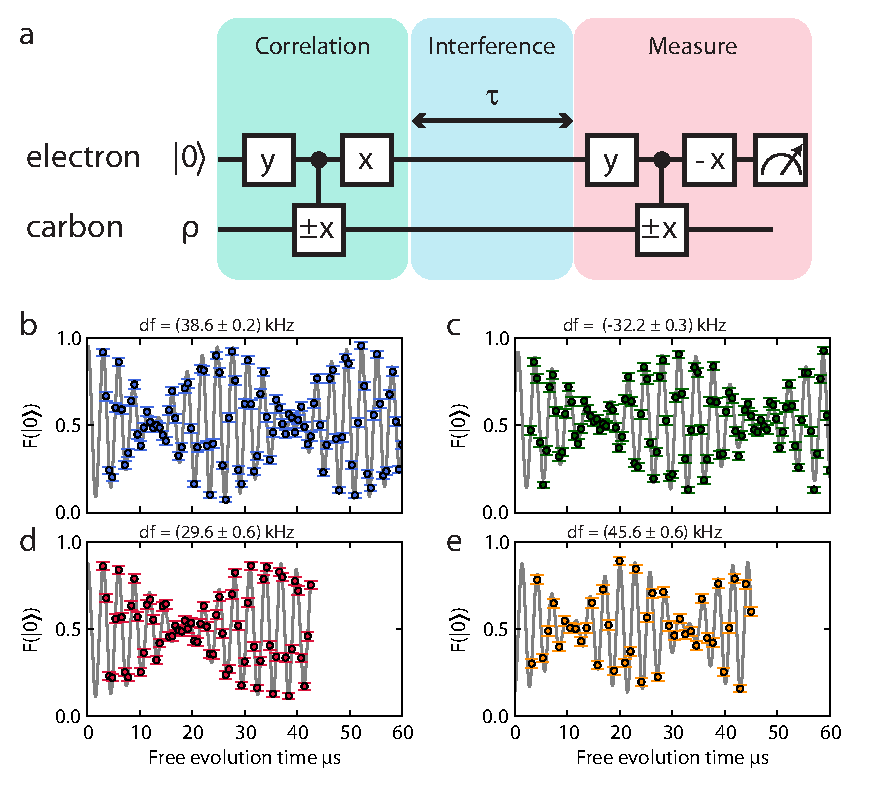
\includegraphics[width=130mm]{Fig2}
	\caption{\label{fig:cdp-fig2} \textbf{Reset of the electron spin} (a) Measurement of the timescale of the reset process. Plotted is the probability of preparing $m_s = 0$ after preparing $m_s = -1$ as a function of repump time and power. Solid lines are fits to the function $S = o - A e^{-\frac{x-x_o}{\tau_{reset}}}-(1-A) e^{-\frac{x-x_o}{\tau_{reset,2}}}$ (b) Largest of the two fitted time constant of the reset process as a function of reset power.}
\end{figure*}

\section{Dephasing of a carbon spin upon optical excitation of the electron spin.}

 We demonstrate the robustness of the carbon spin quantum memory by measuring its ability to store a coherent quantum state while performing the local operations for generating heralded entanglement on the electron spin (Fig. \ref{fig:cdp-fig3}). We prepare carbon spin 1 in a maximum superposition $\ket{\psi}=(\ket{0}_C + \ket{1}_C)/\sqrt{2}$ and perform state tomography after a variable number of protocol repetitions (sequence on electron spin is ($\pi/2 - \pi -$ reset)$^N$, see Fig. \ref{fig:LDE-fig1-protocol}). We omit the two optical $\pi$-pulses to generate spin-photon entanglement. We expect their influence on the carbon spin to be negligible since they effectively perform a measurement of the electron spin which in this case can be incorporated into the reset.
 \begin{figure*}
	\centering
	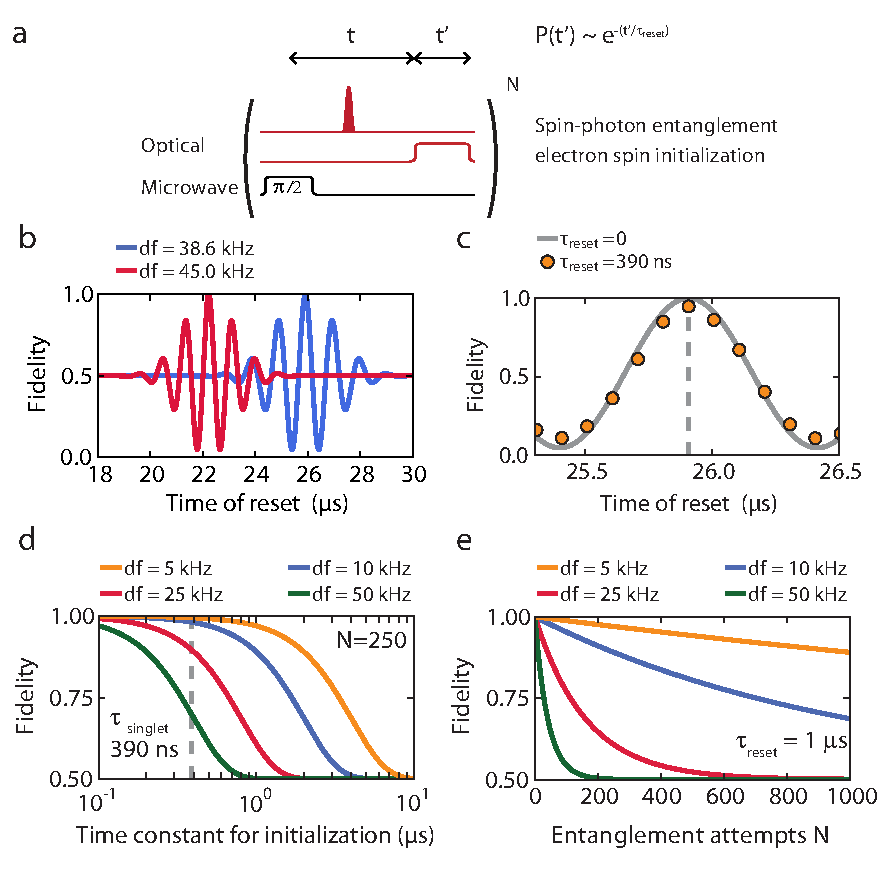
\includegraphics[width=130mm]{Fig3}
	\caption{\label{fig:cdp-fig3} \textbf{} (a) Tomography of carbon spin 1 initially prepared in a superposition as a function of number of repetitions of the heralded entanglement protocol. The repumping pulse is applied for 20 $\mu$s with a power of 100 nW, the time before and after the microwave $pi$-pulse is 200 ns. (b) Dephasing of the carbon spin for different repumping powers, with the same repump time and interpulse delay as in (a). Inset: the decay constants obtained from a fit to the data in (b) as a function of $\tau_{reset}$ for that laser power. }
\end{figure*}

In Fig. \ref{fig:cdp-fig3}a we show that after 200 repetitions the initial state is almost perfectly recovered for 100 nW repump power ($\tau_{reset} = (870 \pm 100)$ ns). The oscillation in the XY-plane of the Bloch sphere is due to the larmor precession of the carbon spin. In a realistic protocol where the number of required repetitions is probabilistic, this oscillation can be correct with real-time feedback. We therefore take the quadratic sum of the expectation values $<X>_C$ and $<Y>_C$ as a figure of merit and find that this quantity is preserved with a fidelity of $(99 \pm 1) \%$ after 200 repetitions.

Strikingly when we plot the full decay curve (Fig. \ref{fig:cdp-fig3}b) we find that the signal is best fitted with a Gaussian as opposed to an exponential function as expected from equation \ref{eq:CDL-deph_an}. Furthermore, while the measured decay constants for variable reset duration (inset of \ref{fig:cdp-fig3}b) can be fitted to the model, they are two orders of magnitude smaller than expected from the independently measured reset time and coupling constant. Since the decoherence rate is also faster than the intrinsic $T_2^{*}$ of the carbon spin, we conclude that the electron reset induces an additional decoherence process that is not included in our model. One hypothesis is that the perpendicular component of the hyperfine interaction ($A_{perp}$, neglected in chapter \ref{ch:CDL}) induces dynamics that lead to a $T_1$-type of decay. This can be verified by measuring the decay of an eigenstate of the carbon spin upon repumping the electron spin. Secondly the model simplifies the spin pumping process which in reality involves multiple transitions in the excited state. 

These experiments establish weakly coupled carbon spins as promising candidates for a memory in a quantum network node based on NV centers. Although further measurements are required to understand the limiting decoherence mechanism, the ability to store a quantum state for hundreds of repetitions can significantly improve the rate at which remote entanglement is established. These results show that in an isotopically purified diamond it is possible to preserve the coherence of a carbon spin during 200 repetitive resets of the electron spin. This is the maximum number of consecutive attempts to generate remote entanglement in previous experiments with NV centers\cite{Bernien_Nature_2013,Pfaff_Science_2014}. However, in protocols that aim to improve the entangling rate by using a quantum memory, the overhead associated with gates on the memory needs to be taken into account. Finding an optimal carbon spin for a quantum memory therefore poses a trade-off between its robustness against optical excitation of the electron spin and the gate-time, since the minimum time required to perform a gate between the nuclear spin and the electron spin is inversely proportional to the coupling strength. Furthermore, all errors in preparing and storing a state in the carbon spin will propagate to the resulting remote entanglement fidelity and therefore the carbon manipulation needs to be improved. In future work the incorporation of a quantum memory in a local node could be combined with the experiments presented in chapter \ref{ch:LDE} to demonstrate entanglement purification\cite{Campbell_Phys.Rev.Lett._2008} and eventually quantum repeaters \cite{Briegel_Phys.Rev.Lett._1998}.

\clearpage
\bibliographystyle{../thesis}
\bibliography{cdp}


